\section{Introduction}

In (typed) functional language we are used to manipulating
structured data by pattern-matching on it.
We include an illustrative example below.

\begin{minipage}{.5\textwidth}

\newcommand{\mknode}[3]{\draw (#1,#2)  circle (.27cm) node[align=center] {\IdrisData{#3}};}
\newcommand{\mkleaf}[2]{\draw[fill=black] (#1,#2) node[align=center] {} +(-.1cm,-.1cm) rectangle +(.1cm,.1cm);}

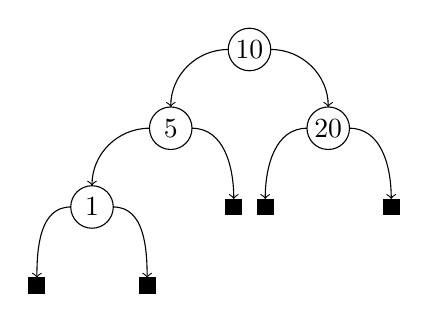
\begin{tikzpicture}
\mknode{0}{0}{10}
  \mknode{-1}{-1}{5};
    \mknode{-2}{-2}{1};
      \mkleaf{-2.7}{-3};
      \mkleaf{-1.3}{-3};
  \mkleaf{-.2}{-2}
  \mknode{1}{-1}{20}
    \mkleaf{.2}{-2}
    \mkleaf{1.8}{-2}

\draw [->] (-0.27,0) to [out=180,in=90] (-1,-.73);
  \draw [->] (-1.27,-1) to [out=180,in=90] (-2,-1.73);
    \draw [->] (-2.27,-2) to [out=180,in=90] (-2.7,-2.9);
    \draw [->] (-1.73,-2) to [out=0,in=90] (-1.3,-2.9);
  \draw [->] (-.73,-1) to [out=0,in=90] (-.2,-1.9);
\draw [->] (0.27,0) to [out=0,in=90] (1,-.73);
  \draw [->] (.73,-1) to [out=180,in=90] (.2,-1.9);
  \draw [->] (1.27,-1) to [out=0,in=90] (1.8,-1.9);
\end{tikzpicture}

\end{minipage}\hfill
\begin{minipage}{.45\textwidth}
  \ExecuteMetaData[Motivating.idr.tex]{motivation}
\end{minipage}

On the left, an example of a binary tree storing bytes in its nodes and
nothing at its leaves.
%
On the right, a small \idris{} snippet defining the corresponding
inductive type and declaring a function summing up all of the
nodes' contents.
%
It proceeds by pattern-matching:
%
if the tree is a leaf then we immediately return 0,
otherwise we start by summing up the left and right subtrees, cast the
byte to a natural number and add everything up.
%
Simply by virtue of being accepted by the typechecker, we know that
this function is covering (all the possible patterns have been handled)
and total (all the recursive calls are performed on smaller trees).

At runtime, the tree will quite probably be represented by
constructors-as-structs and substructures-as-pointers:
%
each constructor will be a struct with a tag indicating which
constructor is represented and subsequent fields will store
the constructors' arguments.
%
Each argument will either be a value (e.g. a byte) or a pointer
to either a boxed value or a substructure.
%
If we were to directly write a function processing a value in this
encoding, proving that a dispatch over a tag is covering, and that
the pointer-chasing is terminating relies on global invariants
tying the encoding to the inductive type.
%
Crucially, the functional language allows us to ignore all of these
details and program at a higher level of abstraction where we can
benefit from strong guarantees.

Unfortunately not all data comes structured as inductive values
abstracting over a constructors-as-structs and substructures-as-pointers
runtime representation.
%
Data that is stored in a file or received over the network is typically
represented in a contiguous format.

We include below a textual representation of the above tree using
\texttt{node} and \texttt{leaf} constructors and highlighting the
data in red.

\medskip
  \texttt{(node (node (node leaf \IdrisData{1} leaf) \IdrisData{5} leaf) \IdrisData{10} (node leaf \IdrisData{20} leaf))}
\medskip

This looks almost exactly like the list of bytes we get when using a
naïve serialisation format based on a left-to-right in-order traversal
of this tree.
%
In the encoding we include below,
leaves are represented by the byte \texttt{00},
and nodes by the byte \texttt{01}
(each byte is represented by two hexadecimal character,
we have additionally once again \IdrisData{highlighted} the bytes
corresponding to data stored in the nodes):

\medskip
\texttt{01 $\overbrace{\texttt{01 $\underbrace{\texttt{01 00 \IdrisData{01} 00}}_{\texttt{(node leaf \IdrisData{1} leaf)}}$
    \IdrisData{05} 00}}^{\texttt{(node (node leaf \IdrisData{1} leaf) \IdrisData{5} leaf)}}$
    \IdrisData{0a} 01 00 \IdrisData{14} 00}
\medskip

The idiomatic way to process such data in a functional language
is to first deserialise it as an inductive type and then call
the \IdrisFunction{sum} function we defined above.
%
If we were using a lower-level language however, we could directly
process the serialised data without the need to fully deserialise it.
%
A basic C implementation of such a sum function could look something
like the following:

\begin{lstlisting}
int sumAt (int buf[], int *ptr, int *acc) {
  int tag = buf[*ptr]; (*ptr)++;
  switch (tag) {
    case 0: return 0;
    case 1:
      sumAt(buf, ptr, acc);
      int val = buf[*ptr]; (*ptr)++;
      *acc += val;
      sumAt(buf, ptr, acc);
      return 0;
    default: exit(-1); }}
\end{lstlisting}


This function takes a buffer, a pointer currently indicating the start of
a tree, and an accumulator in which we add up all the values.
%
We start (line 2) by reading the byte the pointer is referencing and
immediately move the pointer past it.
%
This is the tag indicating which constructor is at the root of the tree
and so we inspect it (line 3).
%
If the tag is 0 (line 4), the tree is a leaf and so we return.
%
If the tag is 1 (line 5), then the tree starts with a node and the rest
of the buffer contains the left subtree, the byte stored in the node,
and then the right subtree.
%
We start by summing the left subtree (line 6),
after which the pointer has been moved past its end and is now pointing
at the byte stored in the node.
We can therefore dereference the byte and move the pointer past it (line 7),
increment the accumulator by the value thus obtained (line 8)
and finally sum the right subtree (line 9).
%
If the tag is anything other than 0 or 1 (line 11) then the buffer does not
contain a valid tree and so we immediately exit with an error code.
%
At the end of a successful run the accumulator contains the sum of the nodes' content.


As we can readily see, this program
directly performs pointer arithmetic,
explicitly mentions buffer reads,
and relies on undocumented global invariants
such as the structure of the data stored in the buffer,
or the fact the pointer is being moved along and points directly past
the end of a subtree once \texttt{sumAt} has finished computing
its sum.

Our goal with this work is to completely hide away all of these
dangerous aspects
and offer the user the ability to program over serialised data
just as seamlessly and correctly as
if they were processing inductive values.
%
We will see that
Quantitative Type Theory (QTT)~\cite{DBLP:conf/birthday/McBride16, DBLP:conf/lics/Atkey18}
as implemented in \idris{}~\cite{DBLP:conf/ecoop/Brady21}
empowers us to do just that purely in library code.

\subsection{Seamless Programming over Serialised Data}\label{sec:seamless}

Forgetting about correctness for now, this can be summed up by the
two following code snippets describing how we can compute the sum
of the values stored in the type of tree we are using as a running
example.

%\noindent
%\begin{minipage}{.4\textwidth}
%  \ExecuteMetaData[SaferIndexed.idr.tex]{tsum}
%\end{minipage}
%\hfill\begin{minipage}{.55\textwidth}
%  \ExecuteMetaData[SaferIndexed.idr.tex]{rsum}
%\end{minipage}


\begin{center}
  \begin{minipage}{.5\textwidth}
    \ExecuteMetaData[SaferIndexed.idr.tex]{rsum}
  \end{minipage}
\end{center}

We reserve for later our detailed explanations of the representations
used in this snippets
(\IdrisType{Pointer.Mu} in \Cref{sec:pointers},
\IdrisFunction{view} in \Cref{sec:dataview}).
%
For now, it is enough to understand that the function
is an \IdrisType{IO} process
inspecting a buffer that contains a tree stored in serialised format
and computing the sum as the pure function seen in the previous section.

In both cases, if we have uncovered a leaf
({\IdrisData{"Leaf"} \IdrisData{\#}} \IdrisKeyword{\KatlaUnderscore{}})
then we return zero,
and if we have uncovered a node
({\IdrisData{"Node"} \IdrisData{\#}} \IdrisBound{l} \IdrisData{\#} \IdrisBound{b} \IdrisData{\#} \IdrisBound{r})
with
a left branch \IdrisBound{l},
a stored byte \IdrisBound{b},
and a right branch \IdrisBound{r},
then we recursively compute the sums for the left and right subtrees,
cast the byte to a natural number and add everything up.
%
Crucially, the two functions look eerily similar, and the one operating on
serialised data does not explicitly perform error-prone pointer arithmetic,
or low-level buffer reads.
%
This is the first way in which our approach shines.

One major difference between the two functions is that
we can easily prove some of the pure function's properties by a structural
induction on the input tree whereas we
cannot prove anything about the \IdrisType{IO} process without first
explicitly postulating the \IdrisType{IO} monad's properties.
%
Our second contribution tackles this issue.

\subsection{Correct Programming over Serialised Data}

We will see that we can refine that second definition to obtain
a correct-by-construction version of
\IdrisFunction{sum}, with almost exactly the same code.

\begin{center}
  \begin{minipage}{.7\textwidth}
    \ExecuteMetaData[SaferIndexed.idr.tex]{csum}
  \end{minipage}
\end{center}

In the above snippet, we can see that the \IdrisType{Pointer.Mu} is indexed
by a phantom parameter: a runtime irrelevant \IdrisBound{t} which has type
(\IdrisType{Data.Mu} \IdrisFunction{Tree}).
%
And so the return type is able to mention the pure \IdrisFunction{Data.sum}
function that consumes inductively defined trees.
%
\IdrisType{Singleton} is, as its name suggests, a singleton type
(cf. \Cref{sec:view}). That is
to say that the natural number we compute is now proven to be equal to the
one computed by the pure \IdrisFunction{sum} function.
%
The implementation itself only differs in that we had to use idiom
brackets~\cite{DBLP:journals/jfp/McbrideP08}, something we will explain
in \Cref{sec:datasingleton}.

In other words, our approach also allows us to prove the functional
correctness of the \IdrisType{IO} procedures processing trees stored
in buffer in serialised format. This is our second main contribution.

\subsection{Generic Programming over Serialised Data}

Last but not least, as Altenkirch and McBride
demonstrated~\cite{DBLP:conf/ifip2-1/AltenkirchM02}:
``With dependently (sic) types, generic programming is just programming:
it is not necessary to write a new compiler each time a useful
universe presents itself.''

In this paper we carve out a universe of inductive types that can be
uniformly serialised and obtain all of our results by generic programming.
%
In practice this means that we are not limited to the type of binary trees
with bytes stored in the nodes we used in the examples above.
%
We include below the type signature of a generic and correct-by-construction
definition of \IdrisFunction{fold} operating on data stored in a buffer
(we will explain how it is defined in \Cref{sec:bufferfold}).

\ExecuteMetaData[SaferIndexed.idr.tex]{foldtype}

This data-genericity is our third contribution.

\subsection{Plan}

In summary, we are going to define a library for the
generic,
seamless,
and correct-by-construction
manipulation of algebraic types in serialised format.


\Cref{sec:desc} introduces the language of descriptions capturing the
subset of inductively defined types that our work can handle.
It differs slightly from usual presentations in that it ensures the
types can be serialised and tracks crucial invariants towards that goal.

\Cref{sec:trees} gives a standard meaning to these data descriptions
as strictly positive endofunctors whose fixpoints give us the expected
inductive types.
%
We will use this standard meaning in the specification layer of our work.

\Cref{sec:hexdump} explores the serialisation format we have picked
for these trees: a depth-first, left-to-right infix traversal of the
trees, with additional information stored to allow for the random access
of any subtree.

\Cref{sec:pointers} defines the type of pointers to trees stored in a
buffer and shows how we can use such pointers to write the corresponding
tree to a file.

\Cref{sec:view} introduces the terminology of \emph{views} and
\emph{singleton} types that is crucial to the art of programming
in a correct-by-construction manner.

\Cref{sec:poking} defines IO primitives that operate on serialised
trees stored in an underlying buffer.
%
They encapsulate all the unsafe low-level operations and offer a
high-level interface that allows users to implement correct-by-construction
procedures.

\Cref{sec:serialising} defines a set of serialisation combinators that
allows users to implement correct-by-construction procedures writing
values into a buffer.

\todo{Add benchmarks?}
